\documentclass{beamer}
%
% Choose how your presentation looks.
%
% For more themes, color themes and font themes, see:
% http://deic.uab.es/~iblanes/beamer_gallery/index_by_theme.html
%
\mode<presentation>
{
  \usetheme{CambridgeUS}      % or try Darmstadt, Madrid, Warsaw, ...
  \usecolortheme{default} % or try albatross, beaver, crane, ...
  \usefonttheme{default}  % or try serif, structurebold, ...
  \setbeamertemplate{navigation symbols}{}
  \setbeamertemplate{caption}[numbered]
} 

\usepackage[english]{babel}
\usepackage[utf8x]{inputenc}
\usepackage{tikz}
\usetikzlibrary{trees}

% Set the overall layout of the tree
\tikzstyle{level 1}=[level distance=3cm, sibling distance=2.5cm]
\tikzstyle{level 2}=[level distance=3.5cm, sibling distance=1.2cm]
\tikzstyle{level 3}=[level distance=3cm, sibling distance=0.6cm]

% Define styles for bags and leafs
\tikzstyle{bag} = [text width=2em, text centered]
\tikzstyle{end} = [circle, minimum width=3pt,fill, inner sep=0pt]

\title{ENGG2430D Tutorial 2}
\author{Zhibo Yang}
\institute{\textit{Department of Information Engineering \\ The Chinese University of Hong Kong}}
\date{\textit{January 21, 2015}}

\begin{document}

\begin{frame}
\titlepage
%\center{\footnotesize{\textit{Acknowledgement: Changkun Jiang}}}
\end{frame}

\begin{frame}{Some Information}

\begin{itemize}
  \item Office location: Room 802, HSH Engineering Building
  \item Office hour: Friday 4:00-5:00 pm
  \item Email: ouyangzhibo@cuhk.edu.hk
  \item Language: English, Mandarin \& \textit{very little} Cantonese
\end{itemize}

\end{frame}

% automatically generated outline.
\begin{frame}{Outline}
  \tableofcontents
\end{frame}

\section{The Binomial Theorem}
\subsection{Introduction}

\begin{frame}{The Binomial Theorem}
    The binomial theorem studies the algebraic expansion of powers of a binomial, i.e.,
    \begin{equation} \label{eq: binomial}
    (x+y)^n, n\in\{0,1,2,3,\cdots\}
    \end{equation}
    \uncover<2->{Simple cases:}
    \begin{eqnarray*}
    	\uncover<2->{n=0:  & (x+y)^0=1\\}
    	\uncover<3->{n=1:  & (x+y)^1=x+y\\}
    	\uncover<4->{n=2:  & (x+y)^2=x^2+2xy+y^2\\}
    	\uncover<5->{n=3:  & (x+y)^3=x^3+3x^2y+3xy^2+y^3\\}
    	\uncover<6->{n=4:  & (x+y)^4=x^4+4x^3y+6x^2y^2+4xy^3+y^4\\}
    \end{eqnarray*}
    \uncover<7->{For a large $n$, expanding (\ref{eq: binomial}) by hand is too tedious. Fortunately, Binomial Theorem gives us the expansion (\ref{eq: binomial}) for any nonnegative integer.}
\end{frame}

\subsection{Formulation}
\begin{frame}{The Binomial Theorem}
    \begin{theorem}
    For any nonnegative integer $n$,
    \begin{displaymath}
    (x+y)^n=\sum_{k=0}^nC_n^k
    %\begin{pmatrix}
    %n\\
    %k
    %\end{pmatrix}
    x^ky^{n-k}
    \end{displaymath}
    where 
    $$C_n^k=\frac{n!}{k!(n-k)!} $$
    \end{theorem}
    \vskip 0.5cm
    Two ways to prove:
    \begin{itemize}
    \item \textbf{Combinatorial proof}
    \item Inductive proof
    \end{itemize}
\end{frame}

\subsection{Combinatorial Proof}
\begin{frame}{$(x+y)^3=1(x+y)(x+y)(x+y)$}
    How to expand it?\\
    - use sequential model\\
    - analogy to tossing a fair coin 3 times
    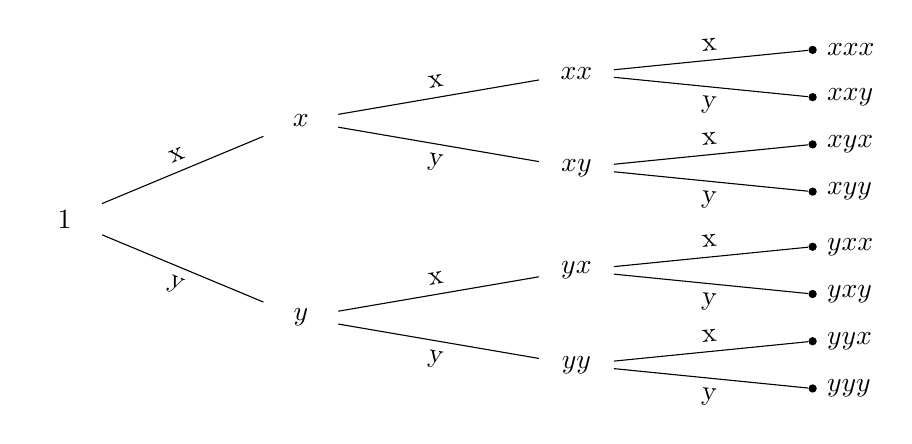
\begin{tikzpicture}[grow=right, sloped]
	\node[bag] {1}
    	child {
        	node[bag] {$y$}        
            child {
            	node[bag] {$yy$} 
            		child{
                			node[end, label=right:
                    		{$yyy$}] {}
                			edge from parent
                			node[above] {}
                			node[below]  {y}
            		}
	   		child{
                			node[end, label=right:
                    		{$yyx$}] {}
                			edge from parent
                			node[above] {x}
                			node[below]  {}
            		}
		edge from parent
	     	node[above] {}
             	node[below]  {y}
	    }
            child {
            	node[bag] {$yx$} 
            		child{
                			node[end, label=right:
                    		{$yxy$}] {}
                			edge from parent
                			node[above] {}
                			node[below]  {y}
            		}
	   		child{
                			node[end, label=right:
                    		{$yxx$}] {}
                			edge from parent
                			node[above] {x}
                			node[below]  {}
            		}
		edge from parent
	    	node[above] {x}
            	node[below]  {}
	    }
	    edge from parent
	    node[above] {}
            node[below]  {y}
    	}
    	child {
        node[bag] {$x$}        
            child {
            	node[bag] {$xy$} 
            		child{
                			node[end, label=right:
                    		{$xyy$}] {}
                			edge from parent
                			node[above] {}
                			node[below]  {y}
            		}
	   		child{
                			node[end, label=right:
                    		{$xyx$}] {}
                			edge from parent
                			node[above] {x}
                			node[below]  {}
            		}
		edge from parent
	    	node[above] {}
             	node[below]  {y}
	    }
            child {
            	node[bag] {$xx$} 
            		child{
                			node[end, label=right:
                    		{$xxy$}] {}
                			edge from parent
                			node[above] {}
                			node[below]  {y}
            		}
	   		child{
                			node[end, label=right:
                    		{$xxx$}] {}
                			edge from parent
                			node[above] {x}
                			node[below]  {}
            		}
		edge from parent
	    	node[above] {x}
             	node[below]  {}
	    }
	edge from parent
    	node[above] {x}
        node[below]  {}
    	};
    \end{tikzpicture}\\
    \textbf{Remark}: Order does not matter, namely, $xxy,xyx,yxx$ are the same. 
    Summing up the leaf nodes, we get $(x+y)^3=x^3+3x^2y+3xy^2+y^3$
\end{frame}

\begin{frame}{Combinatorial proof}
$$(x+y)^n=\underbrace{(x+y)(x+y)\cdots(x+y)}_{\text{n of those}}=\sum_{k=0}^nC_n^kx^ky^{n-k}$$
\begin{itemize}
\item The expansion can be expressed as the sum of multiple items of the form: $a_kx^ky^{n-k}$, $k$ is a nonnegative integer.
\item The expansion is the same with the total sample space of tossing a fair coin $n$ times, $n \ge 1$.
\item Let $x,y$ denote the events "we get a head in one tossing" and "we get a tail in one tossing", respectively. The coefficient $a_k$ in each item equals $C_n^k$ (analogous to the event "in $n$ tossings, we get $k$ heads").
\end{itemize}
\begin{block}{Remarks}
Actually, $n$ does not have to be a nonnegative integer; the binomial theorem can be extended to the power of any real number. 
\end{block}
\end{frame}

\subsection{Applications}
\begin{frame}{Series for $e$}
The Euler's number $e$ is defined as
\begin{displaymath}
e=\lim_{n\to\infty}\bigg(1+\frac{1}{n}\bigg)^n
\end{displaymath}
Applying binomial theorem:
$$\bigg(1+\frac{1}{n}\bigg)^n=1+C_n^1\frac{1}{n}+C_n^2\frac{1}{n^2}+\cdots+C_n^n\frac{1}{n^n}$$
Looking into the $k$th item of the right hand side and take the limit:
$$\lim_{n\to\infty}C_n^k\frac{1}{n^k}=\lim_{n\to\infty}\frac{1}{k!}\cdot\frac{n(n-1)(n-2)\cdots(n-k+1)}{n^k}=\frac{1}{k!}$$
Therefore, $e$ can be written as a series:
$$e=\frac{1}{0!}+\frac{1}{1!}+\frac{1}{2!}+\frac{1}{3!}+\cdots$$
Above is also known as Taylor series of $e^x$ at $x=1$.
\end{frame}

\begin{frame}{Simple Numerical Estimation}
\textbf{Example 1}  \textit{Estimate the value of $1.01^5$ rounding up to 3 decimal places.}\\
\textbf{Solution}:  Using the binomial theorem: let $x=1,y=0.01$,
\begin{displaymath}
\begin{split}
1.01^5 & =(1+0.01)^5\\
& = 1+5(0.01)+10(0.01)^2+10(0.01)^3+5(0.01)^4+(0.01)^5\\
& \approx 1+5(0.01)+10(0.01)^2 = 1.051
\end{split}
\end{displaymath}

\textbf{Example 2}  \textit{Estimate the value of $1.0309^6$ rounding up to 3 decimal places.}\\
\textbf{Solution}:  Again, calculate this by hand will take us some time. But using the binomial theorem, we can try to expand the following
\begin{displaymath}
\begin{split}
(1+x+x^2)^6 & =(1+x(1+x))^6\\
& = 1+6x(1+x)+15x^2(1+x)^2+20x^3(1+x)^3+\cdots\\
& = 1+6x+21x^2+50x^3+\cdots
\end{split}
\end{displaymath}
Let $x=0.03$, we get $1.0309^6\approx1.200$.
\end{frame}

\section{Integer Solutions to Indeterminate Equation}

\subsection{}

\begin{frame}{Integer Solutions to Indeterminate Equation}
\begin{block}{Problem 1}
Suppose we have a equation as follows
$$x_1+x_2+x_3+\cdots+x_n=m$$
where $x_i,n,m$ are positive integers, and $\forall i \in \{1,2,3,4,\cdots,n\}$. Then, how many solutions are there? (hint: use combinations.)
\end{block}
\begin{block}{Solution}
Consider $m$ to be $m$ "1"s summing up together, i.e.,
$$m=\underbrace{1+1+1+\cdots+1}_{\text{m ones}}$$
Every solution of ${x_1,x_2,\cdots,x_n}$ can be matched to an event of selecting $n-1$ "+" between those "1"s.
\end{block}

% Commands to include a figure:
%\begin{figure}
%\includegraphics[width=\textwidth]{your-figure's-file-name}
%\caption{\label{fig:your-figure}Caption goes here.}
%\end{figure}
\end{frame}

\begin{frame}{Integer Solutions to Indeterminate Equation}
Because of the one-to-one matching, the number of solutions is equal to the frequency of the event "picking $n-1$ from $m-1$", that is $C_{m-1}^{n-1}$

\begin{block}{Problem 2}
What if $x_i$ are nonnegative, how many solutions are there? (hint: convert back into the previous problem)
\end{block}
\begin{block}{Solution}
Since $x_i$ can be zero, so for each item we can add 1 to $x_i$. In this way, we can make it positive again. Note that whenever we add 1 in $x_i$, we should also add 1 to the right hand side. Let $x'_i=x_i+1$ which is a positive integer, so the problem is equivalent to $$x'_1+x'_2+x'_3+\cdots+x'_n=m+n$$. So the number of solution is $C_{m+n-1}^{n-1}$
\end{block}
\end{frame}

\begin{frame}
\begin{center}
\huge Thank you!
\end{center}
\end{frame}

\end{document}
